\chapter{Ferramentas existentes e utilizadas}
	%FALTA INSERIR AS IMAGENS DAS IDEs
  \begin{comment}
    Prof. Dr. Ausberto S. Castro Vera
    UENF - CCT - LCMAT - Curso de Ciência da Computação
    Campos, RJ,  2021
    Disciplina: Paradigmas de Linguagens de Programação
    Neste capítulo devem ser apresentadas pelo menos DUAS (e no máximo 5) ferramentas consultadas e utilizadas para realizar o trabalho, e usar nas aplicações. Considere em cada caso:
    \begin{itemize}
        \item Nome da ferramenta (compilador-interpretador)
        \item Endereço na Internet
        \item Versão atual e utilizada
        \item Descrição simples (máx 2 parágrafos)
        \item Telas capturadas da ferramenta
        \item Outras informações
    \end{itemize}
    \section{Editor MNOP}
    \section{Compilador XYZ}
    \section{Interpretador UVW}
    \section{Ambientes de Programação IDE MNP}
  \end{comment}
  Neste capítulo serão apresentadas e ilustradas algumas das ferramentas disponíveis para se utilizar a linguagem R, sendo elas o interpretador R GUI e as IDEs RStudio Desktop, RStudio Cloud, Visual Studio Code e Jupyter Notebook.
  \section{R GUI}
      \begin{itemize}
      	
      	\item \textit{Imagem da ferramenta:}
      	
      	\begin{figure}[H]  \label{RGUI}
      		\centering
      		\caption{R GUI logo após a instalação}
      		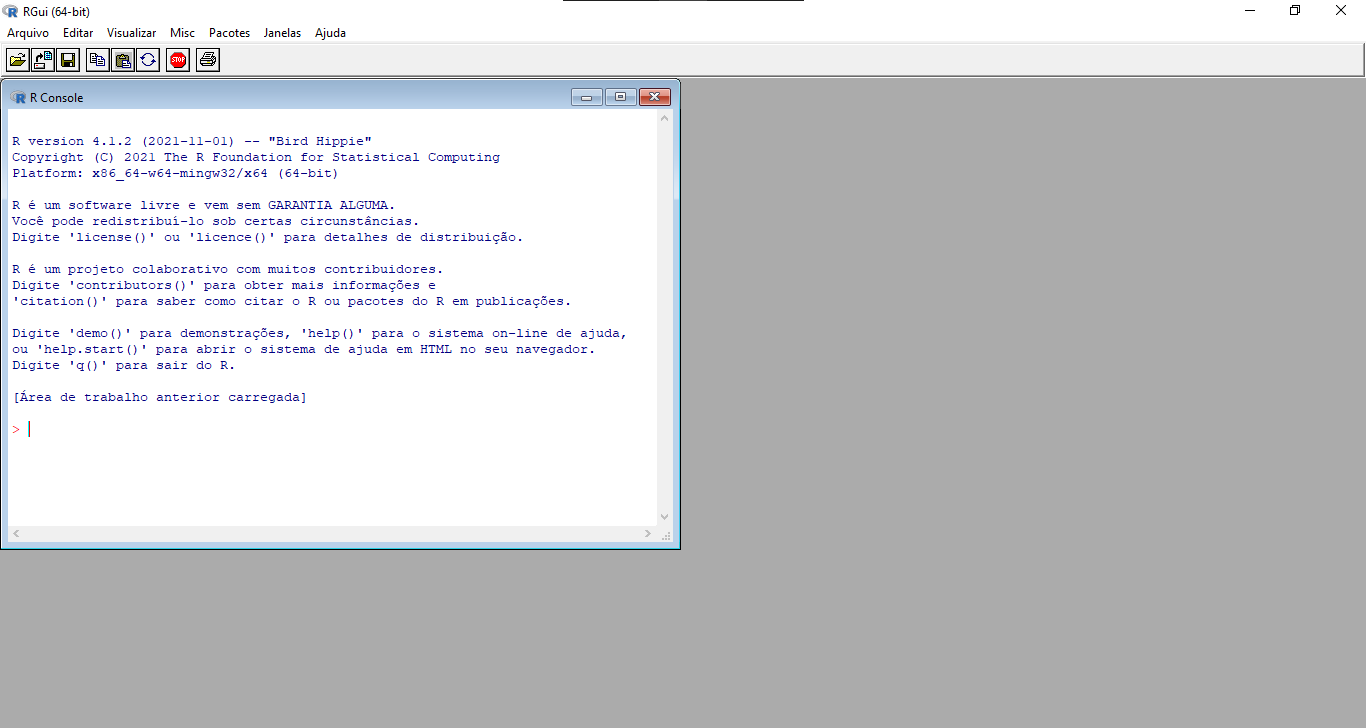
\includegraphics[width=16cm]{PicturesJoaoDias/Ferramentas/RGUI/R_GUI_tela_inicial.png}
      		{\tiny \sf Fonte: autoria própria}
      	\end{figure}
      	
          \item \textit{Link de acesso:} \href{https://cran.rstudio.com/bin/windows/base/}{R GUI} (interpretador)
          \item \textit{Versão:} 4.1.2
          \item \textit{Descrição e comentários:}
            Ferramenta padrão para executar os scripts em R, é interessante pois apresenta algumas demonstrações de coisas que podem ser feitas em R. Executar os códigos nele me pareceu pouco intuitivo. A Figura \ref{RGUI} ilustra a ferramenta logo após a sua instalação.
      \end{itemize}

\newpage
  \section{RStudio Desktop}
    \begin{itemize}
    	
    	\item \textit{Imagem da ferramenta:}
    	
    	\begin{figure}[H]  \label{RStudio_Desktop}
    		\centering
    		\caption{RStudio Desktop logo após a instalação}
    		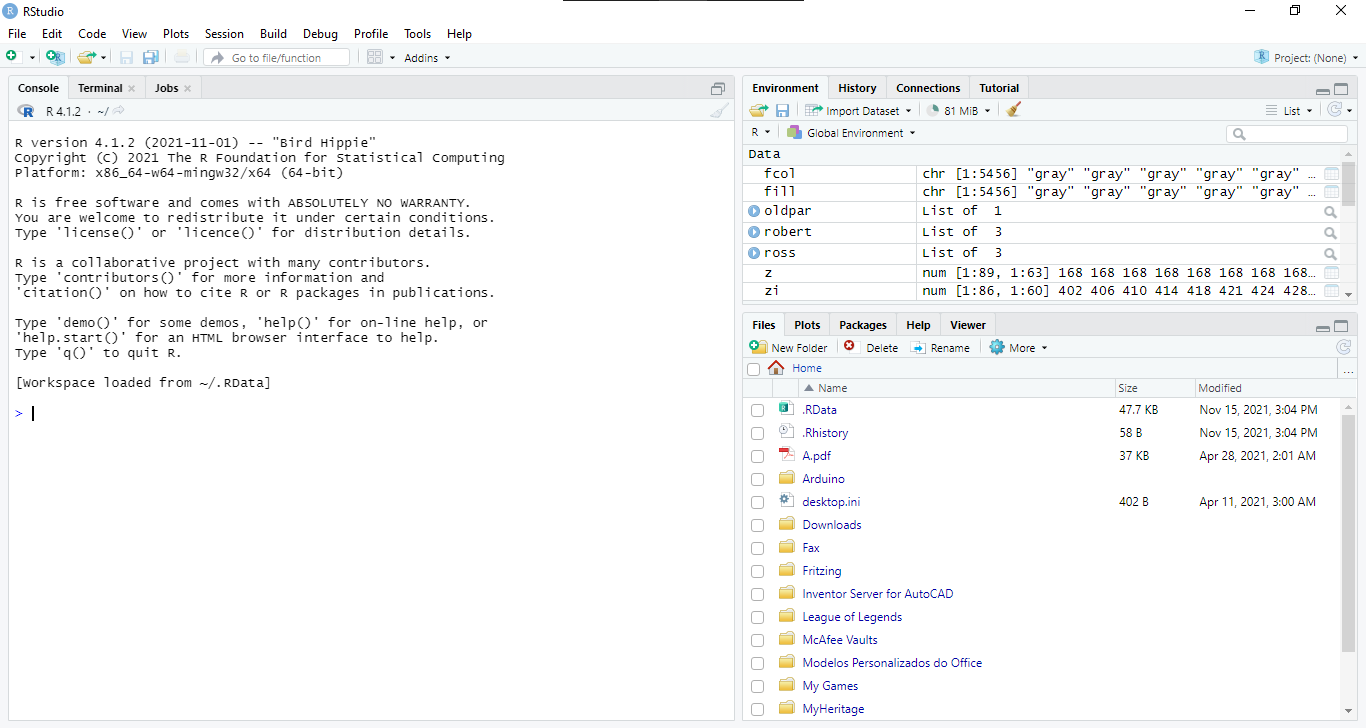
\includegraphics[width=16cm]{PicturesJoaoDias/Ferramentas/RStudio Desktop/RStudio_tela_inicial.png}
    		{\tiny \sf Fonte: autoria própria}
    	\end{figure}
    	
        \item  \textit{Link de acesso:} \href{https://www.rstudio.com/products/rstudio/download/#download}{RStudio Desktop}  (IDE)
        \item \textit{Versão:} 2021.09.1+372 "Ghost Orchid" Release for Windows
        \item \textit{Descrição e comentários:}
          IDE muito utilizada para desenvolvimento de códigos na linguagem R. Inicialmente me senti mais confortável com um ambiente mais moderno e com a possibilidade de configuração de um modo escuro. Há também uma janela que permite seguir tutoriais, o que é bom para iniciantes. Entretanto, assim como no R GUI, não senti que rodar o primeiro código tenha sido intuitivo o bastante. A Figura \ref{RStudio_Desktop} ilustra a ferramenta logo após a sua instalação.
    \end{itemize}
	\newpage
  \section{RStudio Cloud}
      \begin{itemize}
      	
      	\item \textit{Imagem da ferramenta:}
      	
      	\begin{figure}[H]  \label{RStudio_Cloud}
      		\centering
      		\caption{RStudio Cloud logo após a execução}
      		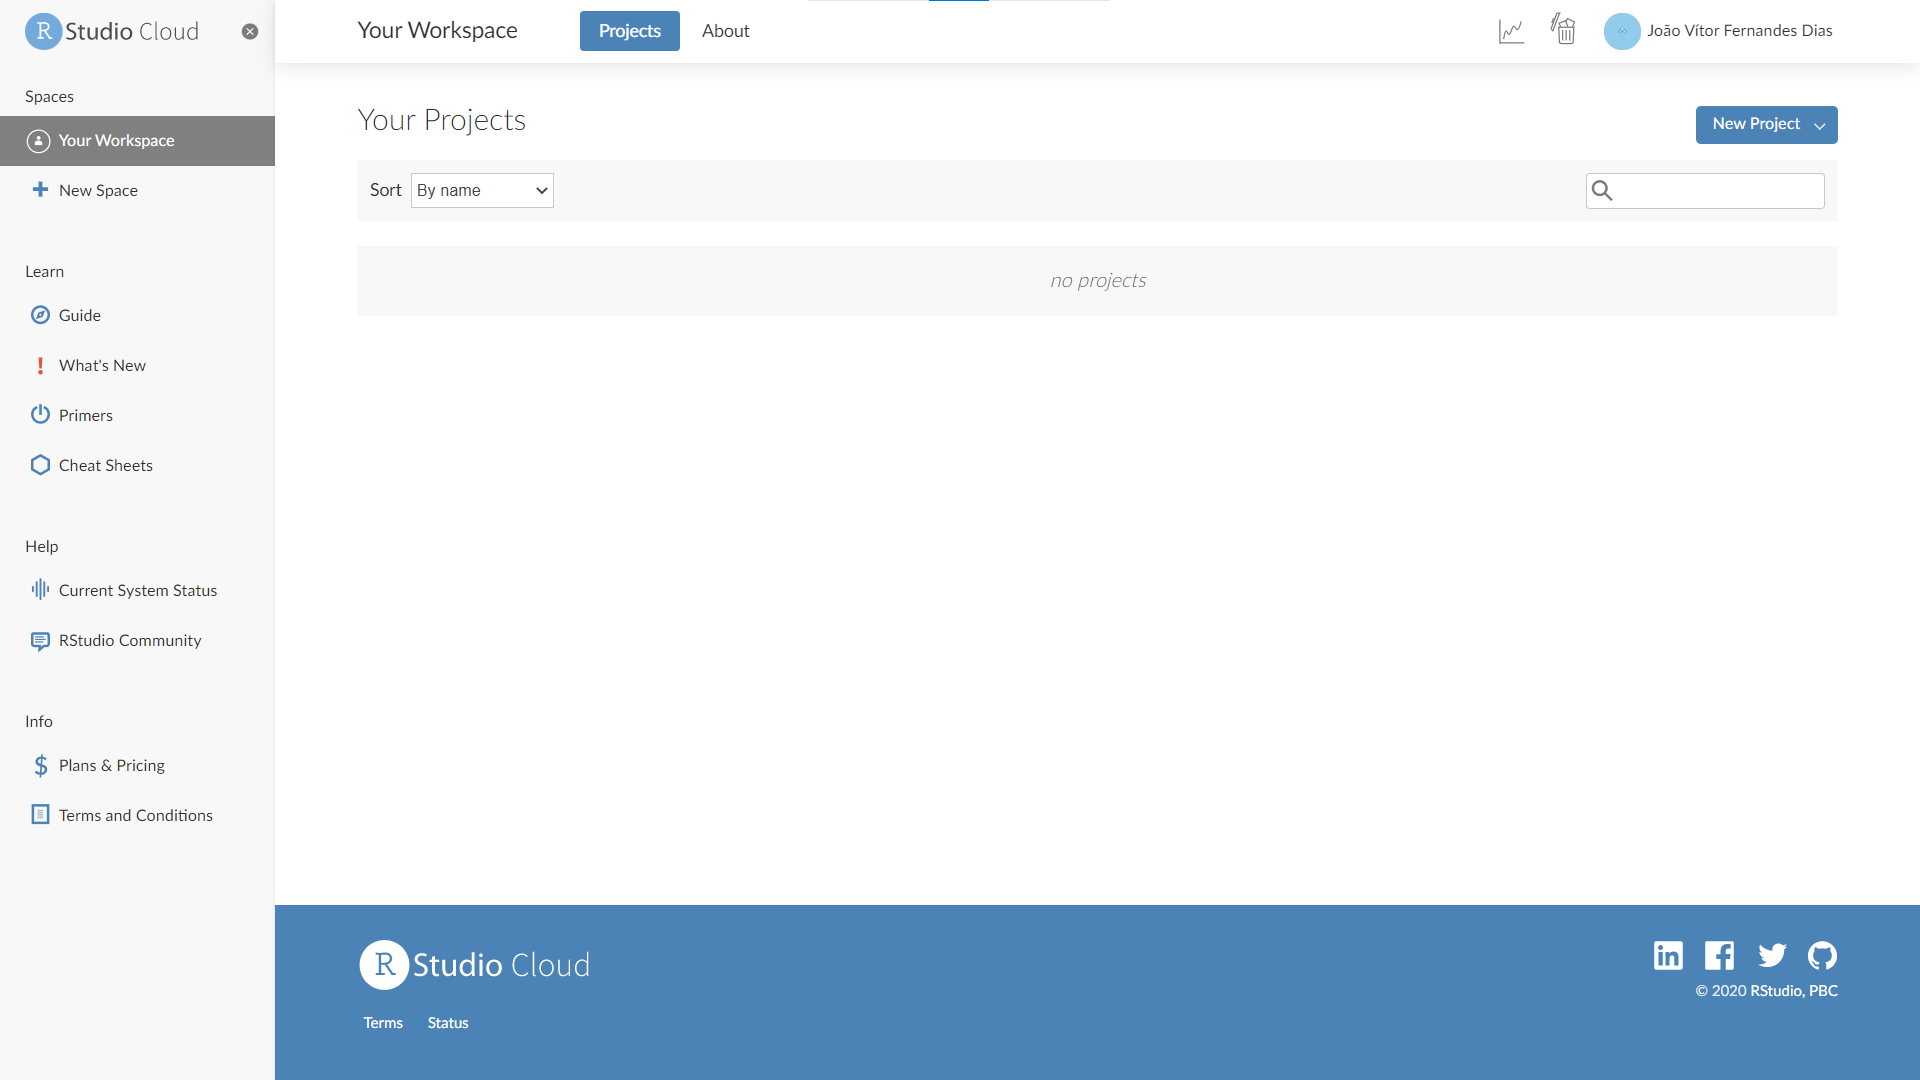
\includegraphics[width=16cm]{PicturesJoaoDias/Ferramentas/RStudio Cloud/RStudio_Cloud_Tela-Inicial.png}
      		{\tiny \sf Fonte: autoria própria}
      	\end{figure}
      	
          \item \textit{Link de acesso:} \href{https://rstudio.cloud/}{URL de acesso ao RStudio Cloud} (IDE e interpretador)
          \item \textit{Versão:} 1.4.1718-1 "Trampled Dandelion" for Ubuntu Bionic

          \item \textit{Descrição e comentários:}
          É bem similar ao RStudio Desktop, só que online e por isso tem a facilidade da portabilidade, mas tem a desvantagem da perda de conexão resultando em pausa no trabalho. Talvez por ter tido contato com o RStudio Desktop antes, a navegação pelo RStudio Cloud me pareceu mais intuitiva. Utilizando do markdown R pude executar o código de forma mais direta. Após essa descoberta no RStudio Cloud, descobri que pode-se usar o R markdown também no RStudio Desktop. Então generalizando, dá para entendermos o RStudio Cloud como sendo um "RStudio Desktop" online. A Figura \ref{RStudio_Cloud} ilustra a ferramenta logo após a sua execução.
      \end{itemize}

\newpage
  \section{Visual Studio Code}
  
  \begin{itemize}
  	
  	\item \textit{Imagem da ferramenta:}
  	
  	\begin{figure}[H]  \label{Visual_Studio_Code}
  		\centering
  		\caption{Visual Studio Code logo após a instalação}
  		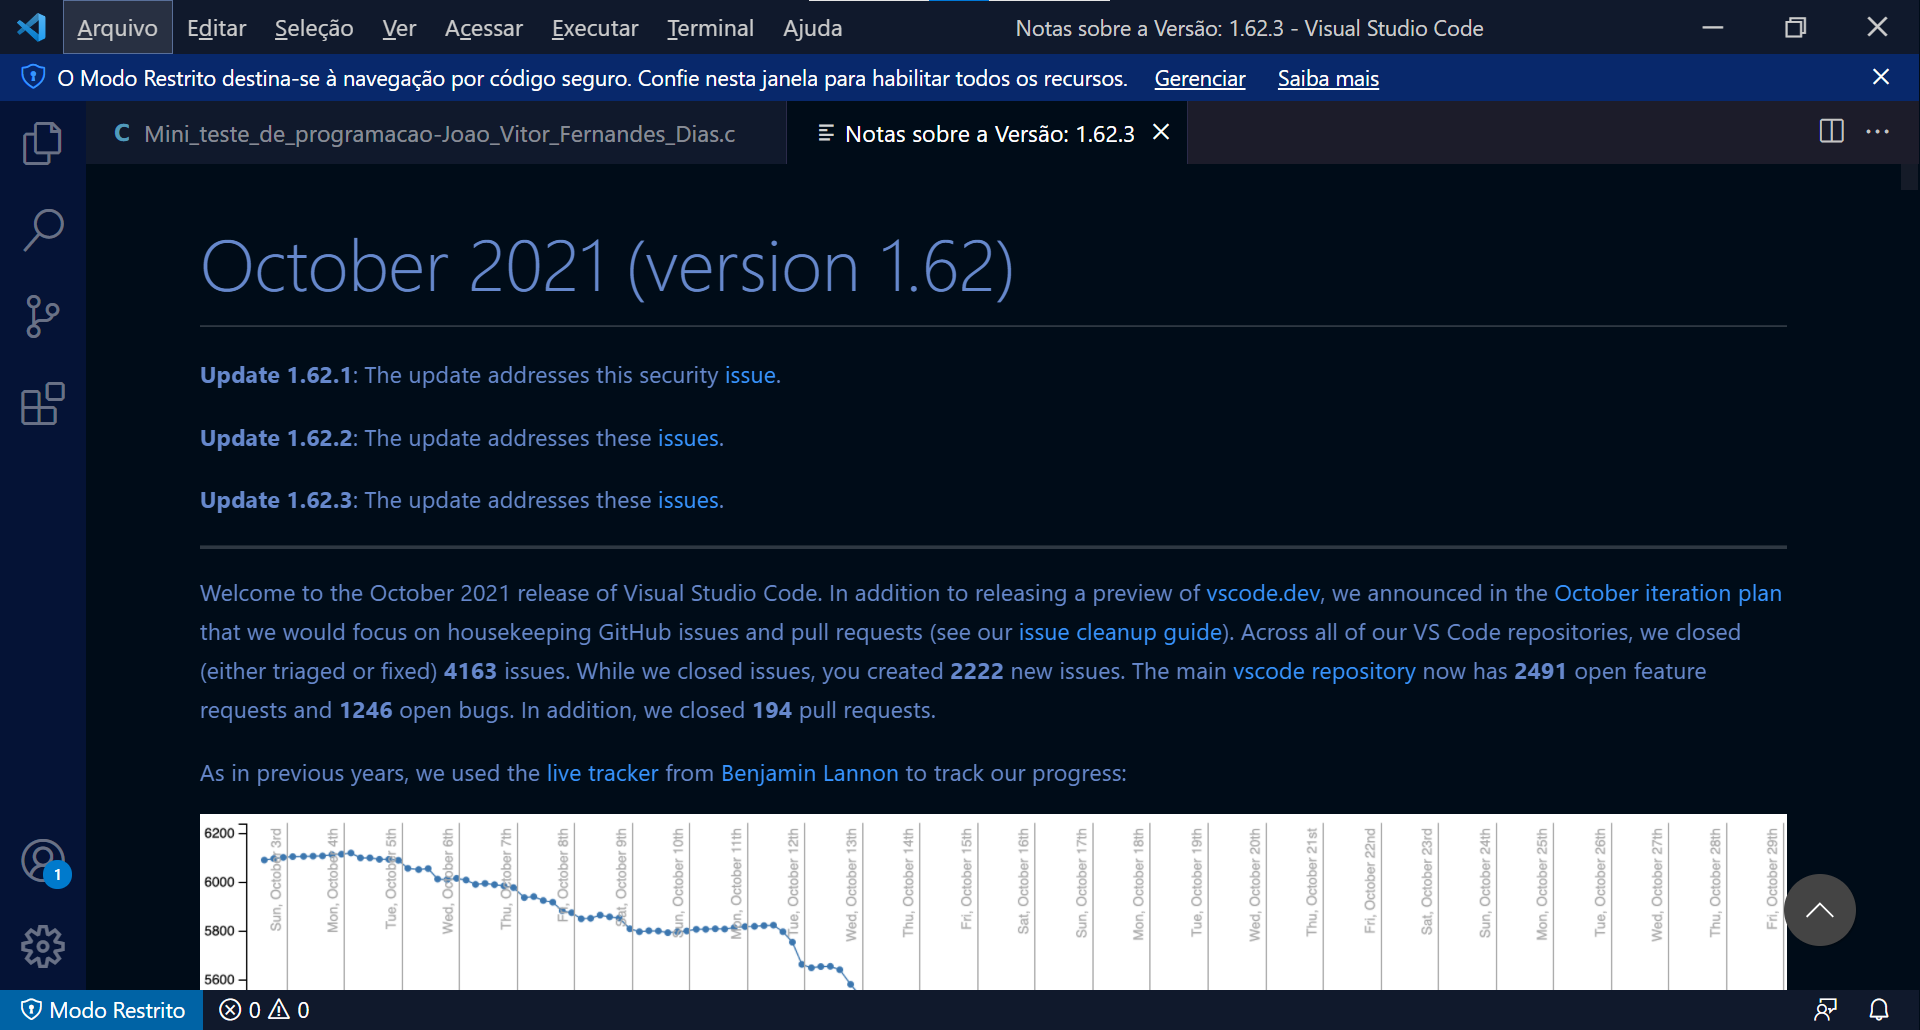
\includegraphics[width=16cm]{PicturesJoaoDias/Ferramentas/Visual Studio Code/Visual_Studio_Code-Tela_Inicial.png}
  		{\tiny \sf Fonte: autoria própria}
  	\end{figure}
  	
  \item \textit{Link de acesso:} \href{https://code.visualstudio.com/docs/?dv=win64}{Visual Studio Code} (IDE)
  	\item \textit{Versão:} 1.62.3
  	\item \textit{Descrição e comentários:}
  	  O Visual Studio Code, ou VSCode ou apenas Code, é uma IDE para programação no geral. É um dos editores de código mais utilizados atualmente, sendo ranqueado como ambiente de desenvolvimento mais popular de 2019 pelo Stack Overflow \cite{Overflow2019}. Quanto ao seu uso para a linguagem R, foi um tanto mais complicado fazê-lo funcionar do que as outras plataformas de desenvolvimento, o que é um ponto negativo. Entretanto, fazer com que o código rodasse foi surpreendentemente mais intuitivo do que nos outros. Como o VSCode pode ser utilizado para várias linguagens diferentes, é uma boa alternativa para quem busca manter todos os ambientes de desenvolvimento em um mesmo lugar. Entretanto, caso seja necessário ferramentas mais específicas do R, o RStudio ainda parece ter maior propriedade. A Figura \ref{Visual_Studio_Code} ilustra a ferramenta logo após a sua instalação.
  \end{itemize}
  		
  		\newpage
  \section{Jupyter Notebook}

  \begin{itemize}
  	
  	\item \textit{Imagem da ferramenta:}
  	
  	\begin{figure}[H]  \label{Jupyter_Notebook}
  		\centering
  		\caption{Jupyter Notebook logo após a execução}
  		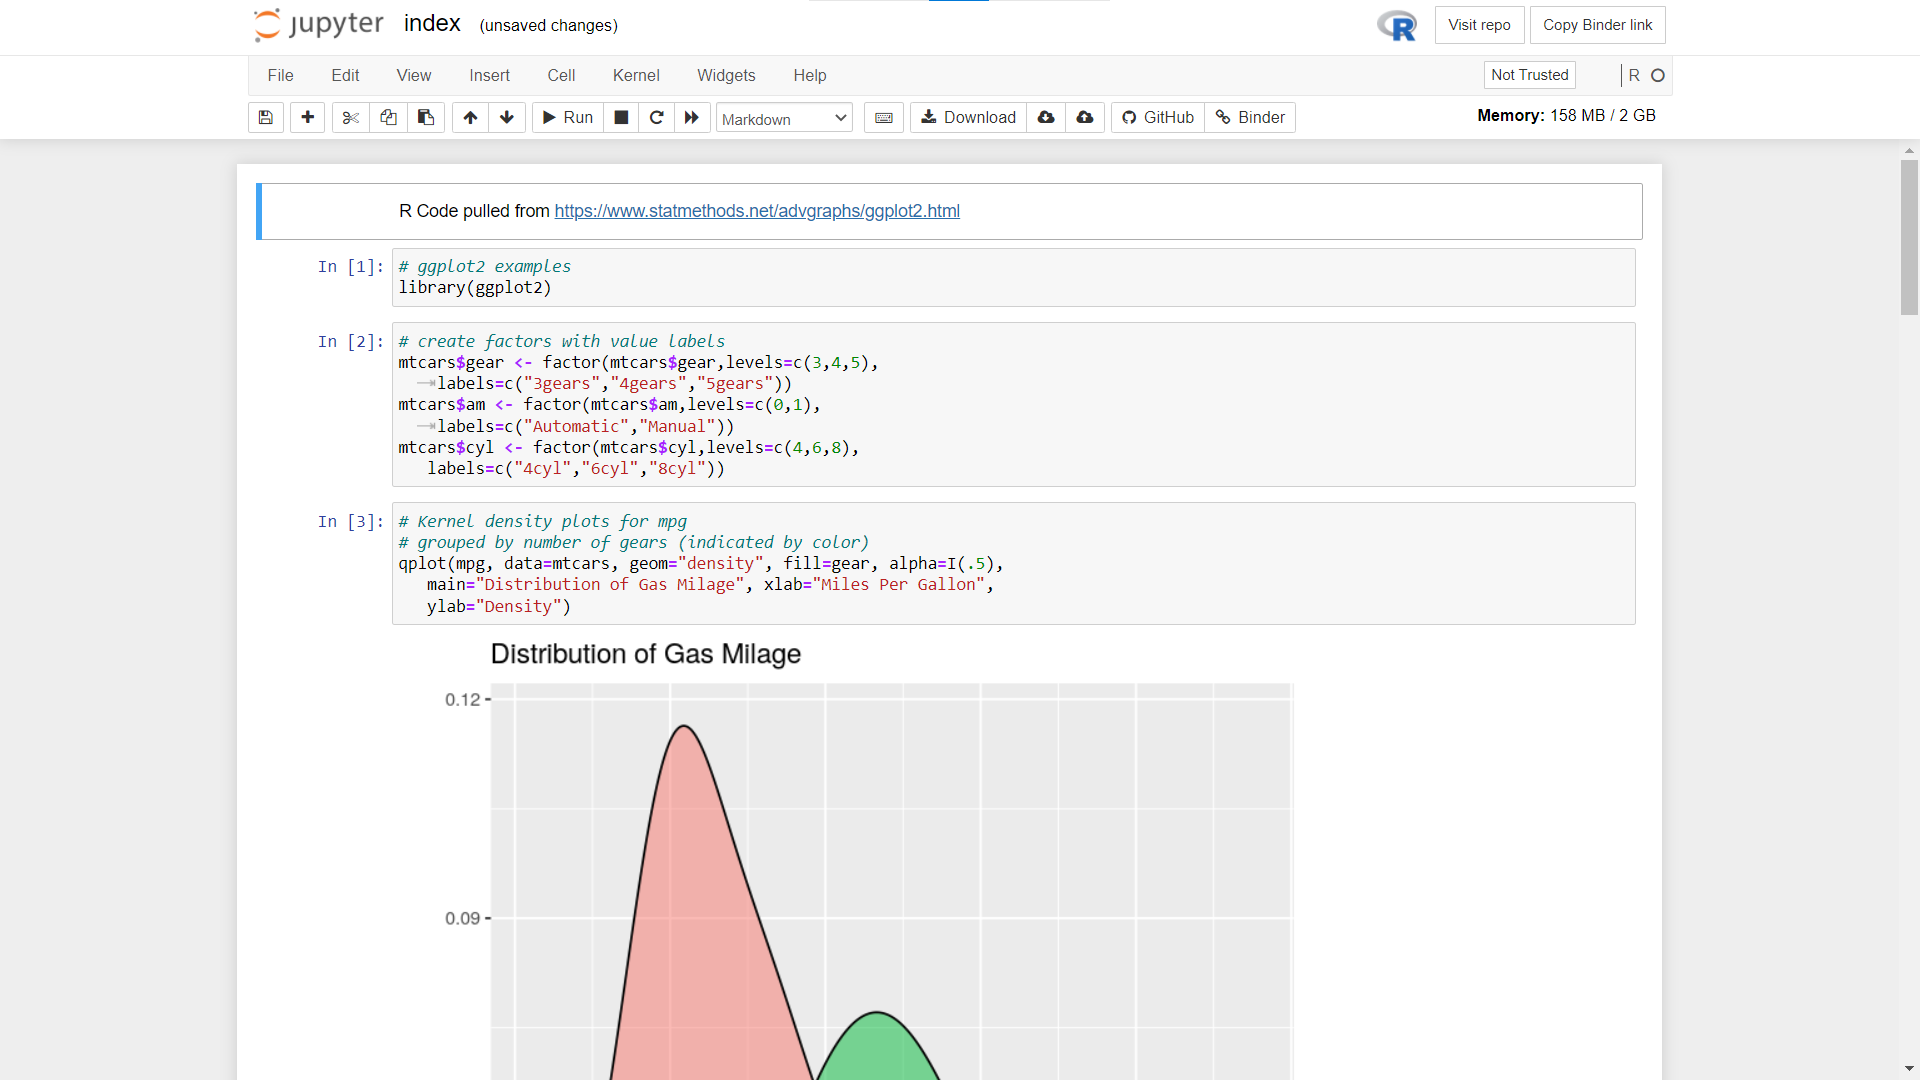
\includegraphics[width=16cm]{PicturesJoaoDias/Ferramentas/Jupyter Notebook/Jupyter_Notebook-Tela_Inicial.png}
  		{\tiny \sf Fonte: autoria própria}
  	\end{figure}
      \item \textit{Link de acesso:} \href{https://mybinder.org/v2/gh/binder-examples/r/HEAD?filepath=index.ipynb}{Jupyter notebook} (IDE e interpretador)
      \item \textit{Versões:}
      \begin{itemize}
          \item Server do notebook: 6.3.0
          \item R: 3.6.3 (2020-02-29)
      \end{itemize}
      \item \textit{Descrição e comentários:}
        Apresenta a mesma estrutura de markdown que o RStudio, porém, por aparentar ter um propósito mais geral abrangendo também códigos Python e Ruby, parece ter menos funcionalidades específicas do R o que torna ela superior na versatilidade de linguagem, mas inferior no propósito específico do uso do R. A Figura \ref{Jupyter_Notebook} ilustra a ferramenta logo após a sua execução.
        
  \end{itemize}
  \section{Resumo}
  	Além das ferramentas citadas aqui, uma maior variedade foi descrita por Milos Gregor \cite{Gregor2018} e pode ser encontrada \href{https://stagraph.com/Post?Id=31&Title=Powered+By+R}{aqui}.
  	
  	Dentre as apresentadas, para decidir de forma mais direta, escolha a IDE se você quer programar:
  	\begin{itemize}
  		\item R GUI: à moda antiga.
  		\item RStudio Desktop: apenas R de modo offline.
  		\item Rstudio Cloud: apenas R de modo online.
  		\item Visual Studio Code: várias linguagens de modo offline.
  		\item Jupyter notebook: várias linguagens de modo online.
  	\end{itemize}
  	\begin{comment}
  		Pode-se substituir a listagem acima por uma tabelinha:
  							Offline			Online
  		Apenas R			RStudio Desktop		RStudio Cloud
  		Várias linguagens	VSCode			Jupyter Notebook
  	\end{comment}